%Je nach dem in welcher Sprache ihr euer Paper schreiben wollt,
%benutzt bitte entweder den Deutschen-Titel oder den Englischen (einfach aus- bzw. einkommentieren mittels '%')

%Deutsch
%\section{Methodischer Ansatz}

%Englisch
\section{Methodological Approach}
This section outlines the methodological approach taken to design, implement, and evaluate an energy-aware server management solution for small and medium-sized enterprises (SMEs).
It describes the overall use case, the technical architecture of the prototype, and the integration of real-time energy consumption and electricity price data.

\subsection{Use Case Description}
This section describes the high-level use case for energy-aware server management in small and medium-sized enterprises (SMEs) with on-premise infrastructure. In this scenario, an SME operates a server infrastructure that supports various business applications. The SME faces the challenge of rising energy costs and seeks to optimize server operations in response to real-time electricity prices.

The main actors in this use case are:
\begin{itemize}
    \item \textbf{SME IT Administrator}: Manages the server infrastructure and monitors energy consumption.
    \item \textbf{Smart Meter}: Measures the total energy consumption of the SME's server room in real time.
    \item \textbf{IoT-Enabled Power Monitoring Devices}: Collect detailed consumption data from individual servers or server racks.
    \item \textbf{Energy Market Data Provider}: Supplies real-time electricity price information (e.g., from EPEX Spot).
    \item \textbf{Energy Management Dashboard}: Aggregates and visualizes consumption and price data, providing actionable insights.    
\end{itemize}

The process begins with the smart meter and IoT devices continuously collecting energy consumption data from the server infrastructure. Simultaneously, the system retrieves real-time electricity prices from the market data provider. The dashboard integrates these data streams, enabling the IT administrator to monitor current consumption, identify high-usage periods, and receive recommendations for optimal workload scheduling. When electricity prices are low, the administrator can schedule energy-intensive tasks (such as backups or batch processing) to minimize costs. Conversely, during peak price periods, non-essential workloads can be deferred. 
\begin{figure}[htbp]
    \centering
    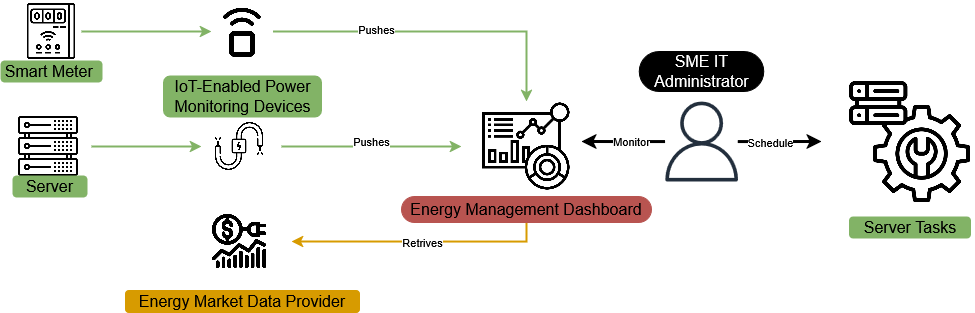
\includegraphics[width=0.8\textwidth]{fig/high_level_use_case.png}
    \caption{Overall Use Case of server admin using the energy management dashboard}
    \label{fig:highleveluse}
\end{figure}
Figure \ref{fig:highleveluse} illustrates the high-level use case, showing the actors and the flow of information. This approach enables SMEs to leverage real-time data and market signals to make informed decisions about server operations, ultimately reducing energy expenses and supporting sustainability goals.

\subsection{Prototype}
The prototype implements a cloud-native architecture that integrates on-premise energy monitoring devices with a suite of scalable AWS services, enabling comprehensive data collection, processing, and visualization tailored for SME server environments. Figure~\ref{fig:architecture} illustrates the system architecture and the flow of information between the various components, serving as the main reference for the following description.

\begin{figure}[htbp]
    \centering
    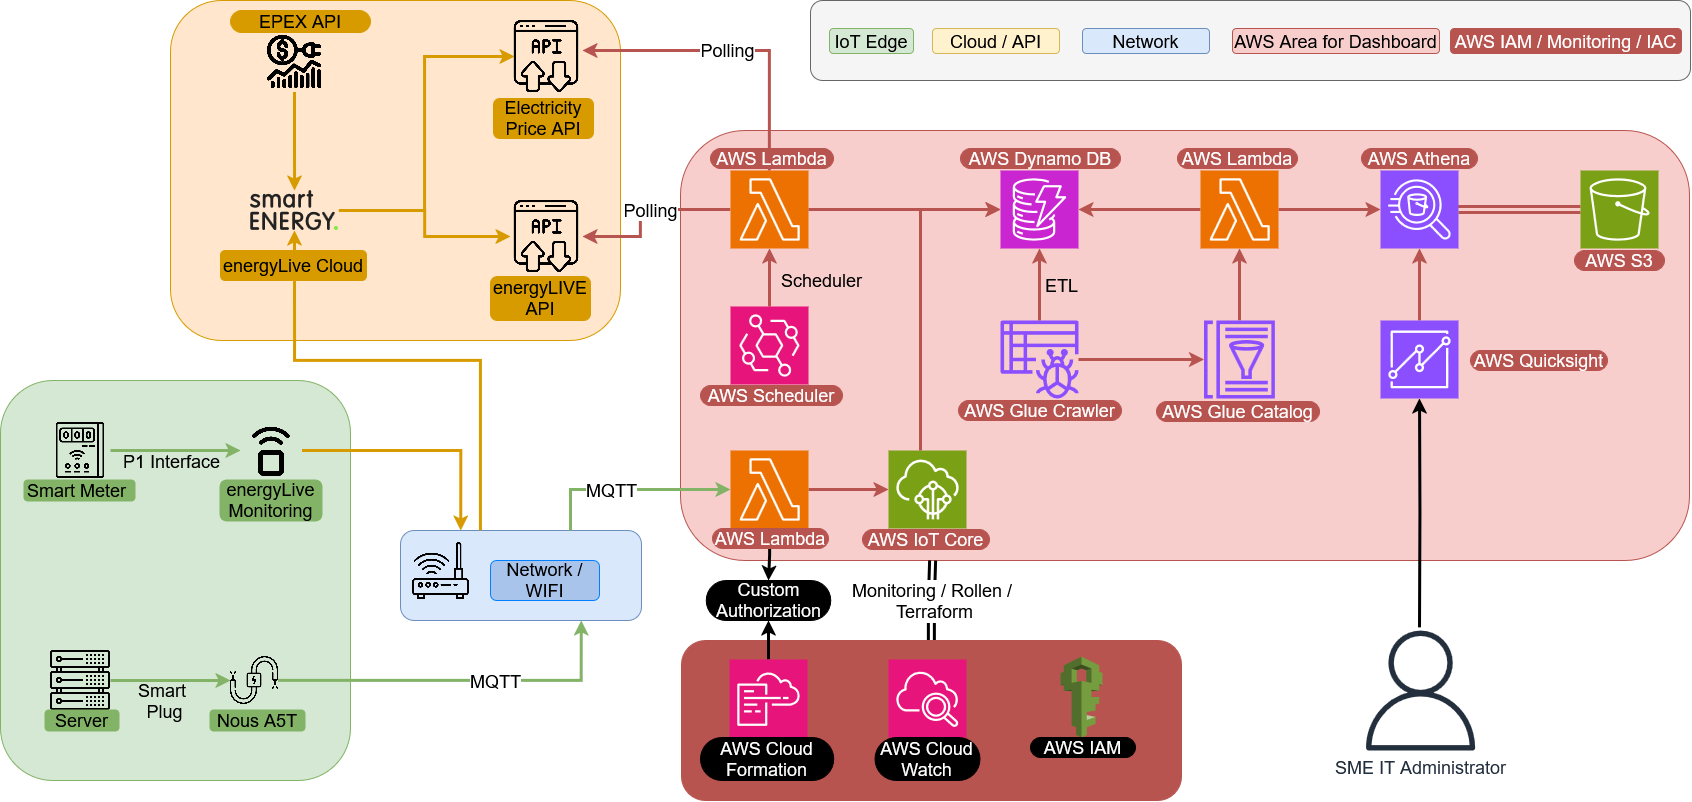
\includegraphics[width=1.2\textwidth]{fig/architektur_new_2.png}
    \caption{System Architecture of the AWS implementation}
    \label{fig:architecture}
\end{figure}

At the edge of the system, a Smart Meter equipped with a P1 interface and the Nous A5T smart plug\footnote{See Appendix~\ref{appendix:tasmota-config} for configuration details and required steps to enable AWS IoT Core integration.} are deployed within the SME's local network. The Smart Meter provides aggregate facility-level energy consumption data, while the Nous A5T device delivers granular, device-specific power usage information. The Smart Meter transmits its data to the energyLive Monitoring platform, which acts as an intermediary for facility-level consumption, whereas the Nous A5T communicates via MQTT over the local WLAN, ensuring real-time reporting of server power usage. These data streams are ingested into the cloud using a combination of polling and message-based mechanisms, reflecting the hybrid nature of the data sources.

The energyLive Cloud platform exposes APIs for both real-time facility consumption (as detailed in Appendix~\ref{appendix:energylive-api}) and electricity market prices (See Appendix~\ref{appendix:strompreis-api} for the electricity price API specification), the latter being sourced from the Strompreis API (EPEX Spot interface). AWS Lambda functions, triggered either by scheduled polling or by incoming MQTT messages, serve as the primary data processing units. This design ensures that both periodic and event-driven data are efficiently captured and processed. The AWS IoT Core service manages secure MQTT communication from the Nous A5T device, while API Gateway and Lambda functions handle RESTful interactions with the energyLive and Strompreis APIs, providing a unified entry point for all external data sources.

All collected data is persistently stored in AWS DynamoDB, which offers a highly available and low-latency database for structured energy and pricing information. To facilitate advanced analytics and reporting, AWS Glue Crawlers and the Glue Catalog automate the extraction, transformation, and cataloging of raw data, making it readily accessible for further analysis. AWS Athena enables ad hoc querying of the curated datasets, while AWS S3 serves as a repository for larger or historical data files, supporting long-term storage and backup requirements. The results of these analyses are presented to users through interactive dashboards built with AWS QuickSight, allowing IT administrators to explore consumption trends, correlate usage with market prices, and identify optimization opportunities in an intuitive manner.

The entire cloud infrastructure is provisioned and managed using AWS CloudFormation, ensuring reproducibility, scalability, and compliance with best practices. Security and operational monitoring are enforced through AWS IAM for access control, CloudWatch for real-time monitoring, and custom authorization mechanisms that safeguard sensitive data flows. This architecture not only provides a robust and scalable foundation for energy-aware server management but also ensures that SMEs can leverage real-time insights and advanced analytics without the need for extensive in-house IT resources. The integration of these components, as depicted in Figure~\ref{fig:architecture}, demonstrates a holistic approach to energy management that is both practical and adaptable to the evolving needs of small and medium-sized enterprises.

\subsection{Evaluation Approach}
To evaluate the effectiveness of our approach, we will implement a comprehensive
evaluation approach that addresses technical performance, server energy
consumption patterns, and economic impacts. This multi-faceted evaluation will
provide insights into both the system's technical capabilities and its practical
utility for SME operators.

Server energy consumption analysis forms the core of our measurement approach.
Using the NOUS A5T PowerCable device, we will conduct detailed measurements of a
single server under various operational scenarios to establish energy consumption
profiles. Specifically, we will examine the following workloads (WL):

\begin{enumerate}[label=WL\arabic*]
    \item \textbf{Maximum computational load:} Simulation of 100\% CPU utilization across all
    cores using the stress-ng tool on a Linux virtual machine. The stress-ng
    command will be configured to spawn CPU-intensive worker processes equal to
    the number of available virtual CPUs, ensuring maximum load across all cores.
    This scenario represents peak computational demand typical of batch processing
    or intensive data analysis tasks. \cite{stressng2020}

    \item \textbf{I/O stress testing:} This WL conduct I/O stress testing to evaluate
    power consumption during intensive disk operations. Using fio (Flexible I/O Tester),
    we will simulate maximum Solid State Drive (SSD) utilization with sequential and random read/write
    patterns. This I/O-intensive scenario represents workloads common in database operations,
    log processing, and large file transfers, providing insights into storage
    subsystem energy requirements under heavy load.

    \item \textbf{System reboot cycle:} Measurement of the overall power consumption profile
    during a full reboot sequence of the host machine, capturing the energy
    requirements during shutdown, boot, and system initialization phases. This
    provides insights into the energy costs associated with maintenance operations
    and system updates.

    \item \textbf{Maintenance operations:} Monitoring of energy consumption during typical
    maintenance activities, specifically the patching process of a Linux virtual
    machine. This scenario represents regular administrative tasks that SMEs must
    perform to maintain security and system integrity.

    \item \textbf{Idle state:} Establishing the baseline energy consumption when the server is
    in an idle state with minimal active processes. This measurement is crucial
    for understanding the fixed energy costs of maintaining server availability
    even during periods of low utilization. \cite{moran2024dissecting,agilewatts2022}
\end{enumerate}

For each WL, the total energy usage consumption will be measured in kilowatt-hours (kWh) and power
consumption patterns over time, establishing detailed energy profiles that can be
correlated with specific operational states. These measurements will reveal the
energy intensity of different server activities and identify potential
optimization opportunities, such as scheduling high-consumption tasks during
periods of lower electricity pricing or implementing more efficient idle-state
management.
\newpage
To ensure reliable and representative measurements, each test scenario will be
conducted with specific time windows (TW):

\begin{enumerate}[label=TW\arabic*]
    \item For maximum computational load and I/O stress testing scenarios, each
    test window will span 15 minutes of load and 15 minutes of idle to capture steady-state 
    behavior and account for any thermal effects or performance throttling that may occur during
    sustained high-load operations.

    \item System reboot cycle measurements will be conducted over multiple
    iterations, with each complete cycle (shutdown to fully operational)
    typically lasting 5-10 minutes, repeated 5 times to ensure consistency and
    account for variations in boot times.

    \item Maintenance operation measurements will cover the entire duration of
    typical update processes, estimated at 5-10 minutes per session, including
    download, installation, and post-update system stabilization periods.

    \item Idle state measurements will be conducted over longer 60-minute windows
    during off-peak hours to establish accurate baseline consumption patterns and
    capture any periodic background system activities.
\end{enumerate}

Each scenario will be repeated three times to ensure statistical validity and
account for any variations in system behavior or environmental conditions. A
minimum cool-down period of 10 minutes will be observed between test iterations
to ensure thermal conditions return to baseline.

\subsection{Test Infrastructure Setup}
To conduct the I/O stress testing scenarios described in WL2, a dedicated test infrastructure in format
of a Ubuntu 24.04.2 LTS virtual machine was established within the Proxmox virtualization environment. 
The test setup addresses the storage space limitations of the primary system disk and ensures 
isolated, reproducible testing conditions.

\subsubsection{Storage Configuration}
The original virtual machine configuration included a 40GB system disk with only 8GB of available
free space, insufficient for intensive I/O testing that requires substantial temporary file creation.
To address this limitation, a dedicated 50GB virtual disk was provisioned and attached to the test
virtual machine as a secondary storage device (\texttt{/dev/sdb}).

The additional disk was formatted with the ext4 filesystem and mounted at \texttt{/mnt/fio-test},
providing 50GB of available space exclusively for I/O testing operations. This configuration
ensures that:

\begin{itemize}
    \item I/O testing operations do not interfere with system operations on the primary disk
    \item Sufficient space is available for creating large test files (up to 32GB total)
    \item Test data can be isolated and cleaned up after each measurement cycle
    \item Storage performance characteristics can be measured independently
\end{itemize}

The disk was configured with I/O threading enabled in the Proxmox hypervisor to maximize I/O
performance and ensure realistic energy consumption measurements under high-load conditions.

\subsubsection{Automated Test Scheduling}
To ensure precise timing alignment with the 15-minute measurement intervals of the energy
monitoring system, automated test scheduling scripts were developed using the \texttt{at}
command scheduler. The FIO stress testing script (\texttt{schedule\_fio\_stress.sh}) implements
the following features:

\begin{itemize}
    \item \textbf{Configurable test cycles:} Support for multiple 15-minute I/O stress periods
    followed by 15-minute idle periods
    \item \textbf{Maximum I/O load generation:} Utilizes 4 parallel FIO jobs with 32-depth I/O queues,
    mixed random read/write patterns (70\% read, 30\% write), and variable block sizes (4KB to 1MB)
    \item \textbf{Direct I/O operations:} Bypasses operating system caches to ensure actual disk I/O
    and realistic power consumption
    \item \textbf{Automatic cleanup:} Removes test files after each cycle to prevent disk space
    exhaustion
    \item \textbf{Comprehensive logging:} Records detailed performance metrics and timestamps
    for correlation with energy measurements
\end{itemize}

This automated approach ensures that I/O stress testing can be precisely 
synchronized with energy measurement intervals, enabling accurate correlation 
between storage workload intensity and power consumption patterns.

\subsubsection{CPU Stress Testing Configuration}
For maximum computational load testing (WL1), a dedicated stress-ng scheduling 
script was developed to generate sustained CPU load across all available cores. 
The stress-ng tool was selected for its ability to create reproducible, 
high-intensity computational workloads suitable for energy consumption analysis.

The CPU stress testing implementation includes the following characteristics:
\begin{itemize}
    \item \textbf{Full CPU utilization:} Spawns worker processes equal to the 
    number of available virtual CPUs (56 logical processors)
    \item \textbf{Sustained load patterns:} Maintains 100\% CPU utilization 
    for the entire 15-minute test duration
    \item \textbf{Thermal consideration:} Includes cooling periods between test 
    cycles to prevent thermal throttling effects
    \item \textbf{Automated scheduling:} Uses the \texttt{at} command for 
    precise timing synchronization with energy measurement intervals
    \item \textbf{Comprehensive logging:} Records CPU utilization metrics and 
    timestamps for correlation with power consumption data
\end{itemize}

The stress-ng configuration utilizes the command 
\texttt{stress-ng --cpu 56 --timeout 900s} to ensure maximum computational 
load across all processor cores. This approach simulates intensive batch 
processing workloads typical in SME environments, such as data analysis, 
compilation tasks, or scientific computing operations.

Similar to the I/O stress testing, the CPU stress script supports configurable 
test cycles with alternating 15-minute stress periods and 15-minute idle 
periods, enabling direct comparison of energy consumption between high-load 
and baseline states. The automated cleanup and logging mechanisms ensure 
consistent test conditions and comprehensive data collection for subsequent 
analysis.

